\documentclass{article}
\usepackage[most]{tcolorbox}
\usepackage{tikz}
\usepackage{graphicx}
\usepackage{lipsum}
\usepackage{amsfonts}
\usepackage{amsthm}
\usepackage{amssymb}
\usepackage[outputdir=../../]{minted}



\newtcolorbox{Qbox}{
enhanced,
colback=white,
}

\newcommand\questionbox[1]{%
  \begin{Qbox}#1\end{Qbox}}

\begin{document}


\subsection*{MAST90084 | Assignment 2}
Author: Sean Conlon, \texttt{sconlon@student.unimelb.edu.au} \\
Student Number: \texttt{1298865}

\vspace{10pt}
\questionbox{\textbf{Question 1.} Prove the various properties outlined in the assignment specification. 
}
\begin{proof}
    If we consider the first property, we have

$$
\begin{aligned}
& \mathbb{E}\left(\frac{\partial \ln f}{\partial \theta_{i j}}\right)=0 \\
& \mathbb{E}\left(\frac{\partial}{\partial \theta_{i j}}\left(y_{i} \theta_{i}-b\left(\theta_{i}\right)\right) \frac{\omega_{i}}{\phi}+c\left(y_{i}, \phi, \omega_{i}\right)\right)=0 \\
& \mathbb{E}\left(\left(y_{i j}-\frac{\partial b\left(\theta_{i}\right)}{\partial \theta_{i j}}\right) \frac{\omega_{i}}{\phi}\right)=0 \\
& \mathbb{E}\left(y_{i j}\right)-\mathbb{E}\left(\frac{\partial b\left(\theta_{i}\right)}{\partial \theta_{i j}}\right)=0 \\
& \mathbb{E}\left(y_{i j}\right)=\frac{\partial b\left(\theta_{i}\right)}{\partial \theta_{i j}}
\end{aligned}
$$

From the second property, we have

$$
\begin{array}{r}
\mathbb{E}\left(\frac{\partial^{2} \ln f}{\partial \theta_{i j} \partial \theta_{i j^{\prime}}}\right)+\mathbb{E}\left(\left(\frac{\partial \ln f}{\partial \theta_{i j}}\right)\left(\frac{\partial \ln f}{\partial \theta_{i j^{\prime}}}\right)\right)=0 \\
\mathbb{E}\left(\frac{\partial}{\partial \theta_{i j}}\left(y_{i j^{\prime}}-\frac{\partial b\left(\theta_{i}\right)}{\partial \theta_{i j^{\prime}}}\right) \frac{\omega_{i}}{\phi}\right)+\mathbb{E}\left(\left(\left(y_{i j}-\frac{\partial b\left(\theta_{i}\right)}{\partial \theta_{i j}}\right) \frac{\omega_{i}}{\phi}\right)\left(\left(y_{i j^{\prime}}-\frac{\partial b\left(\theta_{i}\right)}{\partial \theta_{i j^{\prime}}}\right) \frac{\omega_{i}}{\phi}\right)\right)=0 \\
\mathbb{E}\left(-\frac{\partial^{2} b\left(\theta_{i}\right)}{\partial \theta_{i j} \partial \theta_{i j^{\prime}}} \frac{\omega_{i}}{\phi}\right)+\frac{\omega_{i}^{2}}{\phi^{2}} \mathbb{E}\left(\left(y_{i j}-\mathbb{E}\left(y_{i j}\right)\right)\left(y_{i j^{\prime}}-\mathbb{E}\left(y_{i j^{\prime}}\right)\right)\right)=0 \\
\mathbb{E}\left(\left(y_{i j}-\mathbb{E}\left(y_{i j}\right)\right)\left(y_{i j^{\prime}}-\mathbb{E}\left(y_{i j^{\prime}}\right)\right)=\frac{\phi}{\omega_{i}} \frac{\partial^{2} b\left(\theta_{i}\right)}{\partial \theta_{i j} \partial \theta_{i j^{\prime}}}\right.
\end{array}
$$

So if $j=j^{\prime}$ then

$$
\operatorname{var}\left(y_{i j}\right)=\frac{\phi}{\omega_{i}} \frac{\partial^{2} b\left(\theta_{i}\right)}{\partial \theta_{i j}^{2}}
$$

otherwise,

$$
\operatorname{cov}\left(y_{i j}, y_{i j^{\prime}}\right)=\frac{\phi}{\omega_{i}} \frac{\partial^{2} b\left(\theta_{i}\right)}{\partial \theta_{i j} \partial \theta_{i j^{\prime}}}
$$
\end{proof}

\newpage
\questionbox{\textbf{Question 2.} . You need to install the R package faraway to do this question. The \texttt{hsb} data was collected from the High
School and Beyond Study. Type \texttt{help(hsb)} to see the description of the dataset. We want to see how the
relevant variables in the data are related to the choice of the type of program — academic, vocational, or
general — that the students pursue in high school. The response is multinomial with three levels.
}
\questionbox{\textbf{a)} Fit a trinomial response model with all the other variables other than \texttt{id} as predictors (untransformed). Use “academic” as the base level for the response “prog”. Show the estimated coefficients
and their standard errors.
}

\begin{minted}{r}
    library("faraway")
    library(nnet)
    
    data <- hsb
    # ensure that "academic" is base level
    data$prog <- relevel(data$prog, ref="academic")
    model <- multinom(prog ~ . - id, data=data)
    summary(model)
\end{minted}
Executing the above \texttt{R} script we get the following output for the model summary for covariates and standard errors. Note that for the sake of readability, the below model summary is produced by calling \texttt{print(summary(model),digits=4)}
\begin{center}
    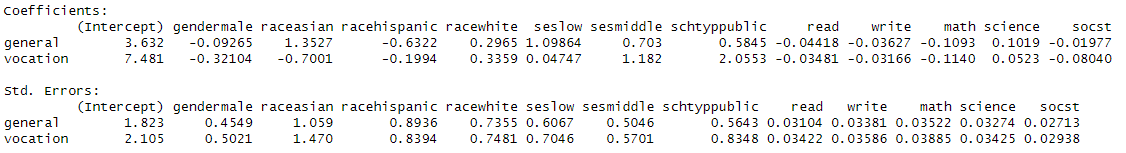
\includegraphics[scale=0.5]{glm-notes/imgs/modelOutput2.PNG}
\end{center}

\questionbox{\textbf{b)} For the student with id \texttt{id}, compute and show the predicted probabilities of the three possible choices.
}
\begin{minted}{R}
    student_99 <- data[data$id == 99, ]
    predicted_probs <- predict(model, newdata = student_99, type = "probs")
\end{minted}
Generates the following outputs for probabilities:
\begin{minted}{R}
    academic   general  vocation 
   0.5076752 0.3753090 0.1170158 
\end{minted}


\newpage

\questionbox{\textbf{Question 3.} In this problem you are to reproduce some of the results in Table 2.7 for Example 2.7 in Fahrmeir and Tutz (F \& T)
}
\questionbox{\textbf{a)} In class, we have reproduced the “robust” p-values shown in the parentheses using the “robust.variance” directly accessible from the gee object produce with the gee() function. For this sub-problem you are asked to compute the robust.variance matrix “by hand”, i.e. using elementary matrix operations in R based on the sandwich-estimator formula. When doing this, you are allowed to use other information accessible from the gee object, such as scale, fitted.values, linear.predictors, residuals, naive.variance, etc. However, you must clearly demonstrate that you can reproduce the robust.variance matrix using the sandwich-estimator formula.}

\begin{minted}{r}
Z <- model.matrix(glm.gee.mu2$terms, data = cells)
sigma <- glm.gee.mu2$scale * exp(glm.gee.mu2$linear.predictors)^2
W <- (glm.gee.mu2$residuals / sigma)^2
D <- exp(glm.gee.mu2$linear.predictors)^2
V <- t(Z) %*% D %*% W %*% Z

B <- glm.gee.mu2$naive.variance
S <- B %*% V %*% B
\end{minted}
The above code derives the \textit{ham} of the sandwich estimator, with the bread being given by \texttt{B <- glm.gee.mu2\$naive.variance}. Using the above code we can reproduce the \texttt{glm.gee.mu2\$robust\_variance} and then :

\begin{minted}{R}
    (Intercept)         TNF         IFN     TNF:IFN 
      0.000            0.000       0.003       0.099 
\end{minted}

\questionbox{\textbf{b)} Now you are to reproduce ALL the numbers presented in the last column of Table 2.7 in F \& T where the variance function is taken to be $\sigma^2(\mu) = \mu+\theta\mu^2$ using the methodology that alternates between estimations of $\theta$ (by method of moments) and $\beta$ (by solving a score equation) we have discussed in lecture.}

\begin{minted}{r}
fit_quasi_likelihood_model <- function(formula, data, max_iter = 100, tol = 1e-6) {
  # initialize estimates
  nb_model <- glm.nb(formula, data=data)
  theta <- nb_model$theta
  
  nb_glm <- glm(formula,
                family = negative.binomial(theta=1/theta),
                data = cells)
  beta <- nb_glm$coefficients
  # Main iteration loop
  for (iter in 1:max_iter) {
    # Update theta using method of moments
    mu <- nb_glm$fitted.values
    theta_new <- sum((nb_glm$residuals^2 - mu)/mu^2)*1/(16-4)
    # Check for convergence
    if (abs(theta_new - theta) < tol) {
      break
    }
    theta <- theta_new
    # Fit a negative binomial model with updated theta
    nb_glm <- glm(formula,
                  family = negative.binomial(theta=1/theta),
                  data = cells)
    beta <- nb_glm$coefficients
  }
  # Return the final model
  return(list(theta = theta, beta = beta, glm = nb_glm))
}

}
\end{minted}
The above function implements the iterative method discussed in the lecture which repeats until convergence in estimate for $\theta$. Call the above function on the appropriate \texttt{model} object we obtain the output:

\begin{minted}{r}
    >theta
    0.21487
\end{minted}
and using the returned \texttt{nb\_glm} object from the function, we can reproduce the robust variance with our model output as before we have
\begin{minted}{R}
    (Intercept)         TNF         IFN     TNF:IFN 
      0.000            0.000       0.003       0.099 
\end{minted}

\end{document}

%family=negative_binomial(1/theta, link=log)
%beta_new = abovefit\$coef